\chapter{Theoretical Background}\label{chapter:background}
\thispagestyle{chapterBeginStyle}
\label{theoretical-background}

\section{Machine Learning}

Machine learning is described as a computer system that can increase its performance in performing a specific task by learning from experiences of similar tasks it has performed in the past (Carbonell, Michalski, and Mitchell \cite{carbonell1983overview}). This definition was formally defined by T. Mitchell in 1997 \cite{mitchell1997machine}, and it is currently the most common definition of machine learning:

\begin{definition}{Machine Learning}
A computer program is said to learn from experience E with respect to some class of tasks T and performance measure P if its performance at tasks in T, as measured by P, improves with experience E.
\end{definition}

Machine learning approaches are often divided into three categories: \textit{Supervised learning}, \textit{Unsupervised learning}, and \textit{Reinforcement learning} \cite{ayodele2010types}. Supervised learning uses labeled training data to approximate the function that maps the input data into correct labels. Unsupervised learning does not use the labeled training data. Instead, it uses the unlabeled data to create a representation of that data, which can then be used for tasks like clustering or as an input for other types of networks. Lastly, reinforcement learning learns decisions by interacting with a dynamic environment. Correct decisions are rewarded, which should encourage the system to make similar decisions.

\vspace{\baselineskip}

This thesis focuses on supervised learning, and to be more specific, the classification task. Classification requires the model to provide a single class based on the input data, whereas regression tries to find the relation between the input and the output. Supervised learning is used in many fields, especially in the image classification task, which base on the set of input features, should infer the correct class of the object on the image.

\section{Neural Networks}\label{section:neural-networks}

\begin{wrapfigure}{R}{0.5\textwidth}
% \vspace{-50mm}
    \centering
  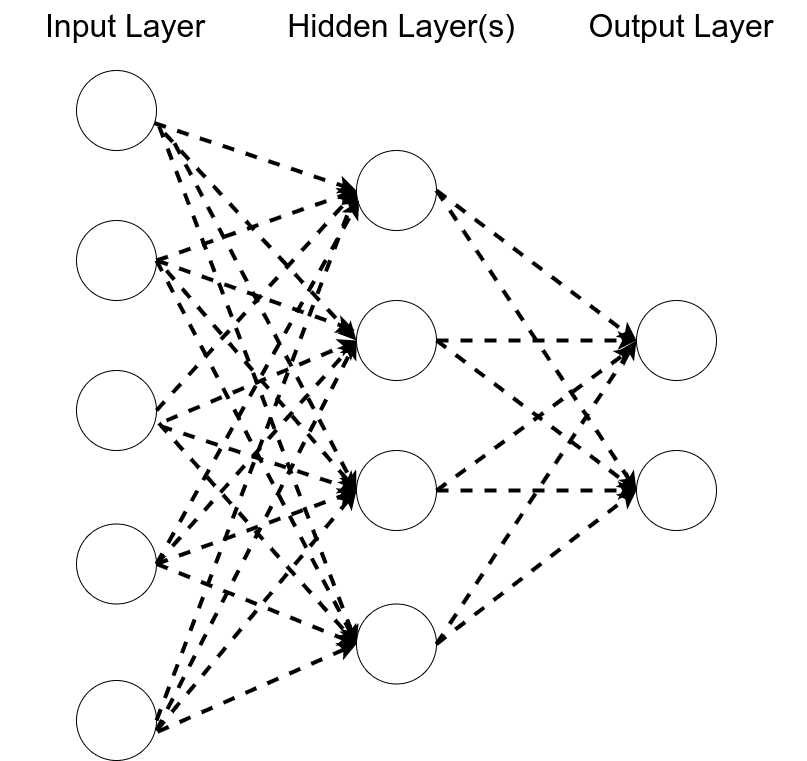
\includegraphics[width=0.45\textwidth]{background/images/neural-network.png}
  \caption{Basic artificial neural network structure.}\label{fig:neural-network}
  \vspace{-16mm}
\end{wrapfigure}

Artificial Neural Networks are systems that are based on the network of neurons of the animal brain \cite{mcculloch1943logical}. These neurons are called \textit{artificial neurons} and are referred to as \textit{nodes}. They are interconnected and organized in \textit{layers} to eventually form a neural network (see Fig. \ref{fig:neural-network}). Each node (represented by a circle) receives the information from the nodes in the previous layer and transmits the new information to the next layer. Input nodes are the exception because they already have the information. New information transmitted by the node is a value from its activation function after receiving all the inputs. The connection between two nodes modifies the output from the lower-layer node before entering the higher-layer node. Most of the networks have an additional bias value for each of the nodes, which can be seen as a regularization parameter. Neural networks have at least three layers: one input layer, one output layer, and at least one hidden layer. The output of the neural network can be defined as:

\begin{equation}\label{eq:forward-pass}
    z^l_j = \sigma \left( \sum_{i}^N(x_i^{l-1} *w_{i,j}^l) + b^l_j \right)
\end{equation}

\newpage

Where:

\begin{itemize}
    \item $l$ is a current layer
    \item $z_j^l$ is an output from the $j$th neuron in layer $l$
    \item $x_i^{l-1}$ is an output from the $i$th neuron on the $l-1$ layer (previous layer)
    \item $w_{i,j}^l$ is a weight for the pair of a current neuron at $j$th position and $i$th neuron from the previous layer
    \item $N$ is a number of neurons in the $l-1$ layer
    \item $b_j^l$ is a bias of $j$th neuron in layer $l$
    \item $\sigma$ is an activation function
\end{itemize}

The goal of a neural network is then finding the value of the weights $w_{ij}^l$ and the biases $b_j^l$ to generate the correct output. These values are optimized in the process called backpropagation.

\subsection{Backpropagation}

Backpropagation is an algorithm that calculates the changes to the weights of the network that are then used to update those weights. The process was first described by Paul Werbos in 1974 \cite{werbos1974beyond}. Even if the name "backpropagation" refers only to gradient computation, it is usually used to describe the whole process of updating the weights. This process consists of three parts. The first part is a feed-forward computation of the input (as defined above), then the error is calculated using the loss function, and lastly, based on the loss function with respect to the weights, the backpropagation computer the gradient used to update the weights.

\vspace{\baselineskip}

After the forward propagation, the error is calculated using a loss function $L(y,\hat{y})$ (where $\hat{y}$ is a predicted output and $y$ is a target output). Usually, the output of the network is a vector $\hat{y} \in \mathbb{R}^n$, and the loss function is a function that translates the difference between $y$ and $y$ into a real number, representing the "cost". One of the simplest loss functions is the Euclidean distance:

\begin{equation}
    L(y,\hat{y}) = \frac{1}{2} || \hat{y} - y  ||^2
\end{equation}

In order to update weights, the gradients have to be calculated with respect to these weights:

\begin{equation}
    \frac{\partial L}{\partial W_l}
\end{equation}

Where $W_l$ is a weight matrix at layer $l$. Computation of that gradient is difficult, but fortunately, the chain rule can be used. It is easier to explain the calculation when the forward function is split into parts (where $\text{CE}$ stands for \textit{Cross-Entropy} loss function defined in equation \ref{eq:cross-entropy}, often used for classification).

\begin{equation}
    z_1 = W_1x + b_1
\end{equation}
\begin{equation}\label{eq:activation-relu}
    h = \text{ReLU}(z_1)
\end{equation}
\begin{equation}
    z_2 = W_2h + b_2
\end{equation}
\begin{equation}
    \hat{y} = \text{sorfmax}(z_2)
\end{equation}
\begin{equation}
    L = \text{CE}(y, \hat{y})
\end{equation}

\begin{equation}\label{eq:cross-entropy}
    \text{CE}(y, \hat{y}) = -(y log(\hat{y}) + (1-y)log(1-\hat{y}))
\end{equation}


Gradient for $W_1$:

\begin{equation}
    \frac{\partial L}{\partial W_1} = \frac{\partial L}{\partial z_2}\frac{\partial z_1}{\partial W_1} = \left( (\hat{y} - y)^Tz_2 \circ sgn(h) \right)^T x^T
\end{equation}

And for $b_1$ :

\begin{equation}
    \frac{\partial L}{\partial w_1} = \frac{\partial L}{\partial z_2}\frac{\partial z_1}{\partial b_1} = \left( (\hat{y} - y)^Tz_2 \circ sgn(h) \right)^T
\end{equation}

Where $sgn$ is a sign function which is a derivative of the ReLU activation function (see eq. \ref{eq:relu-deriv}). With the value of the gradients, weights and biases can be updated.

\subsubsection*{ReLU}

\begin{wrapfigure}{R}{0.30\textwidth}
  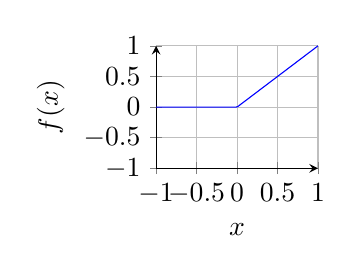
\begin{tikzpicture}
    \begin{axis}[
        axis lines = left,
        xlabel = $x$,
        ylabel = {$f(x)$},
        width=0.3\textwidth,
        ymin = -1,
        ymax = 1,
        grid=both,
        legend pos=north east,
    ]
    %Here the blue parabloa is defined
    \addplot [
        domain=-1:1, 
        samples=100, 
        color=blue,
        ]
        {max(0, x)};
    
    \end{axis}
  \end{tikzpicture}
  \caption{$\text{ReLU}(x)$ where $x \in <-1,1>$}\label{fig:relu-example}
  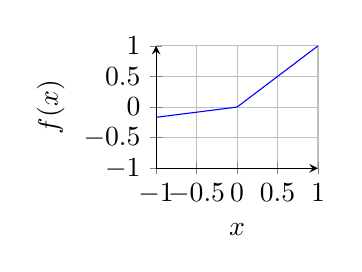
\begin{tikzpicture}
    \begin{axis}[
        axis lines = left,
        xlabel = $x$,
        ylabel = {$f(x)$},
        width=0.3\textwidth,
        ymin = -1,
        ymax = 1,
        grid=both,
        legend pos=north east,
    ]
    %Here the blue parabloa is defined
    \addplot [
        domain=-1:1, 
        samples=100, 
        color=blue,
        ]
        {max(x/6, x)};
    
    \end{axis}
  \end{tikzpicture}
  \caption{$\text{Leaky ReLU}(x)$ where $x \in <-1,1>$}\label{fig:leaky-relu-example}
\end{wrapfigure}

As described in equation \ref{eq:forward-pass} and then later in \ref{eq:activation-relu}, the output is calculated with the use of the activation function. Usually that function is a ReLU function \cite{hahnloser2000digital}. ReLU stands for \textit{Rectified Linear Unit function} and is defined as:

\begin{equation}
    \text{ReLU}(x) = max(x,0)
\end{equation}

and visualized in Figure \ref{fig:relu-example}. Because ReLU returns $0$ every time the value of $x$ is less than $0$, it can deactivate neurons, and therefore create sparser networks. There are two issues with the ReLU function. The first one is that it can create "dead neurons" if all of the inputs of a neuron are less than zero. The second one is that it is not fully differentiable (at the $(0,1)$ point). The first one was solved by Mass et al. \cite{maas2013rectifier} by replacing a zero-valued tail of the ReLU with a slightly negative value $\alpha x$ (where $\alpha$ is a small positive number). Derivative of the ReLU function is defined as follow:

\begin{equation}\label{eq:relu-deriv}
    \text{ReLU}'(x) = \begin{cases} 1 & \text{if } x > 0 \\ 0 & \text{otherwise} \end{cases} = sgn(\text{ReLU}(x))
\end{equation}

\subsection{Convolutional Neural Networks}

Convolutional Neural Network (CNN) \cite{lecun1995convolutional, lecun1989backpropagation} are the type of Neural Networks with at least one convolutional layer. The first convolutional neural networks were LeNet \cite{cnnLecun1998} and AlexNet \cite{krizhevsky2012imagenet}, using only a few convolutional layers. CNNs are assuming that the input data consists of hierarchical patterns which can be used instead of relying on individual features and creating a connection between every single feature and neuron. This approach helps to reduce the number of parameters required by the network.

\subsubsection*{Convolutional Layer}

The convolutional layer uses the idea of filters/kernels with a given size and depth. A layer like that produces the output called a feature map, which is a combination of all the outputs from the kernels. As mentioned, each kernel is defined by the size (which corresponds to its width and height), depths (usually the depth of the input), and additional parameters like padding, stride, or dilatation. The name "convolutional" comes from the mathematical operation of convolution, which is denoted by $f*g$, and the output of that operation is a function that described how one function modifies the other. It can be defined as:

\begin{equation}
    g(m,n) = (h*f)(m,n) = \sum_{u} \sum_{v} h(u,v)f(m-u,n-v)
\end{equation}

Where $f$ is the input image, $h$ is the kernel, $m$ and $n$ are the corresponding row and column in the feature map, and $u$ and $v$ range over all legal subscripts for $h(u,v)$ and $f(m-u,n-v)$ \cite{keller2010convolutions}. An example of the convolution operation for the $m=0, n=3$ is shown in Figure \ref{fig:convolutional operation}.

\begin{figure}[ht]
    \centering
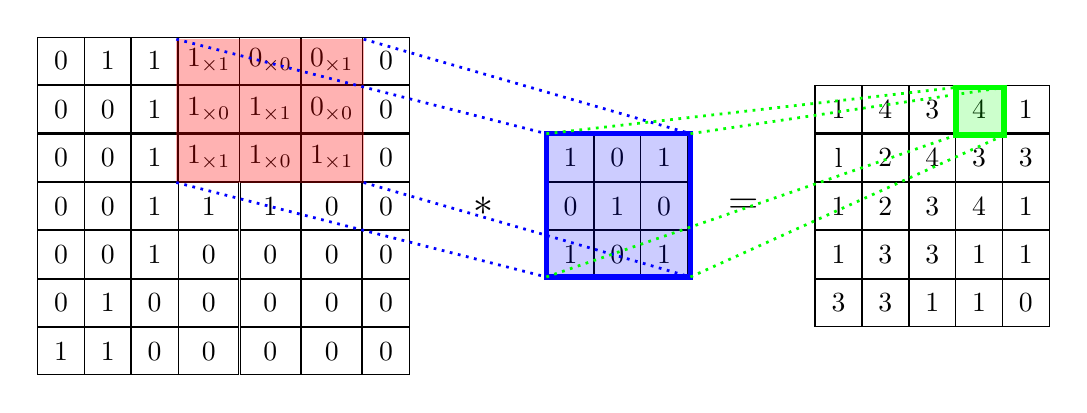
\begin{tikzpicture}[scale=1.0]

  \matrix [nodes=draw,column sep=-0.2mm, minimum size=6mm]
  {
    \node {0}; & \node{1}; & \node {1}; & \node{$1_{\times 1}$}; & \node{$0_{\times 0}$}; 
    & \node{$0_{\times 1}$}; & \node{0}; \\
    \node {0}; & \node{0}; & \node {1}; & \node{$1_{\times 0}$}; & \node{$1_{\times 1}$}; 
    & \node{$0_{\times 0}$}; & \node{0}; \\
    \node {0}; & \node{0}; & \node {1}; & \node{$1_{\times 1}$}; & \node{$1_{\times 0}$}; 
    & \node{$1_{\times 1}$}; & \node{0}; \\
    \node {0}; & \node{0}; & \node {1}; & \node{\, 1 \,}; & \node{\, 1 \, }; 
    & \node{\, 0 \,}; & \node{0}; \\
    \node {0}; & \node{0}; & \node {1}; & \node{\, 0 \, }; & \node{\, 0 \, }; 
    & \node{\, 0 \,}; & \node{0}; \\
    \node {0}; & \node{1}; & \node {0}; & \node{\, 0 \, }; & \node{\, 0 \, }; 
    & \node{\, 0 \,}; & \node{0}; \\
    \node {1}; & \node{1}; & \node {0}; & \node{\, 0 \,}; & \node{\, 0 \, }; 
    & \node{\, 0 \,}; & \node{0}; \\
  };


  % coordinates for coloring filter in array
  \coordinate (A) at (-0.6,0.3);
  \coordinate (B) at (1.78,0.3);
  \coordinate (C) at (1.78,2.12);
  \coordinate (D) at (-0.6,2.12);
  \fill[red, opacity=0.3] (A)--(B)--(C)--(D)--cycle;
  \begin{scope}[shift={(3.3,0)}]
    \node[] at (0,0) {\Large $\ast$};
  \end{scope}[shift={(2.5,0)}]

  \begin{scope}[shift={(5,0)}]

    %\matrix [matrix of math nodes,left delimiter={[},right
    %delimiter={]}]
    \matrix [nodes=draw,column sep=-0.2mm, minimum size=6mm]
    {
      \node{1};  & \node{0};   & \node{1};  \\
      \node{0};  & \node{1};   & \node{0};  \\
      \node{1}; & \node{0}; & \node{1}; \\
    };
    \coordinate (A1) at (-0.9,-0.9);
    \coordinate (B1) at (0.93,-0.9);
    \coordinate (C1) at (0.93,0.92);
    \coordinate (D1) at (-0.9,0.92);
    \fill[blue, opacity=0.2] (A1)--(B1)--(C1)--(D1)--cycle;
    \draw[blue, line width=2] (A1)--(B1)--(C1)--(D1)--cycle;
  \end{scope}

  \draw[dotted, line width=1, color=blue] (A)--(A1);
  \draw[dotted, line width=1, color=blue] (B)--(B1);
  \draw[dotted, line width=1, color=blue] (C)--(C1);
  \draw[dotted, line width=1, color=blue] (D)--(D1);

  \begin{scope}[shift={(6.6,0)}]
    \node[] at (0,0) {\Large $=$};
  \end{scope}[shift={(2.5,0)}]

  \begin{scope}[shift={(9,0)}]

    %\matrix [matrix of math nodes,left delimiter={[},right
    %delimiter={]}]
    \matrix [nodes=draw,column sep=-0.2mm, minimum size=6mm]
    {
      \node{1};  & \node{4};   & \node{3}; & \node{4}; & \node{1};  \\
      \node{l};  & \node{2};   & \node{4}; & \node{3}; & \node{3};  \\
      \node{1}; & \node{2}; & \node{3}; & \node{4} ; & \node{1};  \\
      \node{1}; & \node{3}; & \node{3}; & \node{1} ; & \node{1};  \\
      \node{3}; & \node{3}; & \node{1}; & \node{1} ; & \node{0};  \\
    };
    \coordinate (A2) at (0.3,0.9);
    \coordinate (B2) at (0.91,0.9);
    \coordinate (C2) at (0.91,1.507);
    \coordinate (D2) at (0.3,1.507);
    \fill[green, opacity=0.2] (A2)--(B2)--(C2)--(D2)--cycle;
    \draw[green, line width=2] (A2)--(B2)--(C2)--(D2)--cycle;
  \end{scope}

  \draw[dotted, line width=1, color=green] (A1)--(A2);
  \draw[dotted, line width=1, color=green] (B1)--(B2);
  \draw[dotted, line width=1, color=green] (C1)--(C2);
  \draw[dotted, line width=1, color=green] (D1)--(D2);
\end{tikzpicture}
    \caption{Example of the convolutional operation}
    \label{fig:convolutional operation}
\end{figure}

The standard convolutional layer uses multiple kernels at once, and every one of them has $\text{size} \times \text{size}$ learnable parameters. Putting that in a context where a fully connected neural network requires a weight for every pixel of the input image times the number of neurons in the hidden layer, a convolutional layer is a huge decrease in the total number of parameters. A kernel with a size of $3$ has $9$ learnable parameters. Even with having 50 kernels in the convolutional layer, there are only $450$ learnable parameters in total (for any input image size). For a $32\times32$ image, a fully connected layer with 10 neurons would require $10240$ parameters. It is worth noticing that kernels do not have to be square. The square is computationally efficient, but there were tries to use different shapes \cite{luo2019hexagonal, graham2015sparse, thomas2019kpconv}.

\subsubsection*{Pooling Layer}

CNNs have an additional type of layer called the \textit{Pooling Layer}. There are two types of pooling layers called: \textit{Max Pooling} and \textit{Average Pooling}. Each pooling layer is defined by its size (called the window size), and the result is based only on pixels from that window. The value returned by the max pooling layer is the maximum value from the window. The average pooling layer returns the average from all values from that window.

\begin{figure}[ht]
    \centering
    \begin{subfigure}{.49\textwidth}
        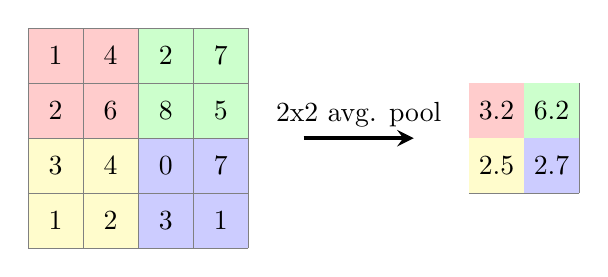
\begin{tikzpicture}[scale=0.7]
        \fill[yellow!20] (0,0) rectangle (2,2);
        \fill[red!20] (0,2) rectangle (2,4);
        \fill[green!20] (2,2) rectangle (4,4);
        \fill[blue!20] (2,2) rectangle (4,0);
        %...
        \draw[gray,very thin] (0,0) grid (4,4);
        \node at (0.5,0.5) {1};
        \node at (1.5,0.5) {2};
        \node at (2.5,0.5) {3};
        \node at (3.5,0.5) {1};
        \node at (0.5,1.5) {3};
        \node at (1.5,1.5) {4};
        \node at (2.5,1.5) {0};
        \node at (3.5,1.5) {7};
        \node at (0.5,2.5) {2};
        \node at (1.5,2.5) {6};
        \node at (2.5,2.5) {8};
        \node at (3.5,2.5) {5};
        \node at (0.5,3.5) {1};
        \node at (1.5,3.5) {4};
        \node at (2.5,3.5) {2};
        \node at (3.5,3.5) {7};
        %...
        \draw[-stealth,ultra thick] (5,2) --node[above] { 2x2 avg. pool} (7,2);
        \draw[gray,very thin] (8,1) grid (10,3);
        \fill[yellow!20] (8,1) rectangle (9,2);
        \fill[red!20] (8,2) rectangle (9,3);
        \fill[green!20] (9,2) rectangle (10,3);
        \fill[blue!20] (9,1) rectangle (10,2);
        \node at (8.5,1.5) {2.5};
        \node at (9.5,1.5) {2.7};
        \node at (8.5,2.5) {3.2};
        \node at (9.5,2.5) {6.2};
        
        \end{tikzpicture}
    \caption{Average Pooling}
    \label{fig:cnn-avg-pooling}
    \end{subfigure}
    \begin{subfigure}{.49\textwidth}
        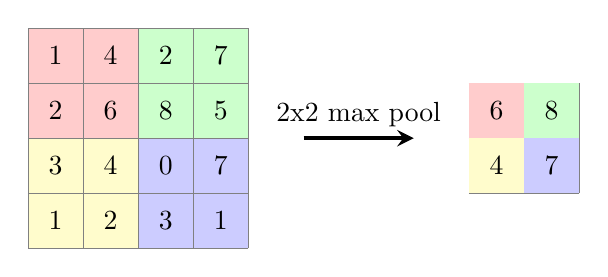
\begin{tikzpicture}[scale=0.7]
        \fill[yellow!20] (0,0) rectangle (2,2);
        \fill[red!20] (0,2) rectangle (2,4);
        \fill[green!20] (2,2) rectangle (4,4);
        \fill[blue!20] (2,2) rectangle (4,0);
        %...
        \draw[gray,very thin] (0,0) grid (4,4);
        \node at (0.5,0.5) {1};
        \node at (1.5,0.5) {2};
        \node at (2.5,0.5) {3};
        \node at (3.5,0.5) {1};
        \node at (0.5,1.5) {3};
        \node at (1.5,1.5) {4};
        \node at (2.5,1.5) {0};
        \node at (3.5,1.5) {7};
        \node at (0.5,2.5) {2};
        \node at (1.5,2.5) {6};
        \node at (2.5,2.5) {8};
        \node at (3.5,2.5) {5};
        \node at (0.5,3.5) {1};
        \node at (1.5,3.5) {4};
        \node at (2.5,3.5) {2};
        \node at (3.5,3.5) {7};
        %...
        \draw[-stealth,ultra thick] (5,2) --node[above] { 2x2 max pool} (7,2);
        \draw[gray,very thin] (8,1) grid (10,3);
        \fill[yellow!20] (8,1) rectangle (9,2);
        \fill[red!20] (8,2) rectangle (9,3);
        \fill[green!20] (9,2) rectangle (10,3);
        \fill[blue!20] (9,1) rectangle (10,2);
        \node at (8.5,1.5) {4};
        \node at (9.5,1.5) {7};
        \node at (8.5,2.5) {6};
        \node at (9.5,2.5) {8};
        
        \end{tikzpicture}
    \caption{Max Pooling}
    \label{fig:cnn-max-pooling}
    \end{subfigure}
    \caption{Example of pooling layers results applied to the same $4 \times 4$ feature map. Colors indicate the area from which the values are pulled to produce the result.}
    \label{fig:cnn-pooling}
\end{figure}
\section{Interpretability}\label{section:interpretability-def}

There is no one formal definition of interpretability and/or explainability in the context of machine learning, and often it is used interchangeably \cite{guidotti2018survey}. Arrieta et al. \cite{arrieta2020explainable} distinguish between the two and define them as:

\begin{definition}[Interpretability]\label{def:interpretability}
Passive characteristic on a model refers to the level of understanding of the models' internal decision process for a human observer.
\end{definition}

\begin{definition}[Explainability]\label{def:explainability}
Active characteristic of a model, associated with the notion of explanation of the action or procedure taken by the model with the intent of clarifying its internal decision process.
\end{definition}

The name of the field Explainable Artificial Intelligence (XAI) refers to the characteristic of a model, but any representation presented to the human (like input attribution) refers to the interpretability of the model. This thesis focuses on the interpretability of CNNs and uses the taxonomy of interpretability as defined in Figure \ref{fig:taxonomy-interpretability} \cite{lipton2018mythos}.

\subsection{Taxonomy of interpretability}\label{section:taxonomy-xai}

\begin{figure}[ht]
    \centering
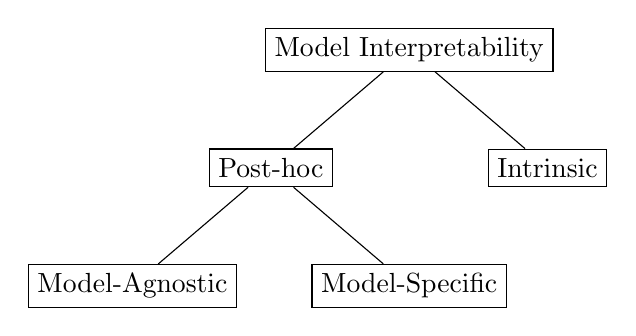
\begin{tikzpicture}[sibling distance=10em,
  every node/.style = {shape=rectangle,
    draw, align=center,
    top color=white, bottom color=white}]]
  \node  {Model Interpretability}
      child { node {Post-hoc}
        child { node {Model-Agnostic} }
        child { node {Model-Specific} } }
      child { node {Intrinsic} };
\end{tikzpicture}
    \caption{Taxonomy of the model interpretability.}
    \label{fig:taxonomy-interpretability}
\end{figure}

There are two major types of models: \textit{white-box models} and \textit{black-box models}. Interpretability of the first type is defined as the \textit{Intrinsic} \cite{biran2017explanation}. This type of interpretability covers all models which have an interpretable internal structure. As an example, the structure of a decision tree is considered interpretable, as well as the internal structure of a shallow neural network. This does not apply to deep neural networks where \textit{post-hoc} interpretability is used. The post-hoc interpretability means that we are trying to explain a prediction of the model without explaining the exact internal mechanism of that model. Because of the complexity of CNNs, post-hoc interpretability is the only way to interpret this kind of model.

\begin{remark}
This is not the only taxonomy of interpretability. The structure of the interpretability can be defined in many ways (either by the purpose, by the method, or by the application).
\end{remark}

\subsubsection*{Model-Agnostic and Model-Specific}

As shown in the taxonomy (see Fig. \ref{fig:taxonomy-interpretability}), post-hoc interpretability is divided into \textit{model-agnostic} and \textit{model-specific} \cite{adadi2018peeking}. The model-agnostic methods are the methods that can be applied to any black-box model without the concern about the internal structure of the model. These methods are usually less precise but because they explain the models' behavior only based on the input and the output. On the other hand, model-specific methods are associated with a particular type of model. The "type" is loosely defined and can refer to the whole domain like CNNs or the specific architecture of CNN. In this thesis, both types of post-hoc interpretability are used.

\subsection{Right to explanation}

The "right to explanation" is a term used by the European Parliament and Council in the General Data Protection Regulation (GDPR) \footnote{Reg (EU) 2016/679 of the European Parliament and of the Council of 27 April 2016 on the protection of natural persons with regard to the processing of personal data and on the free movement of such data, and repealing Dir 95/46/EC (General Data Protection Regulation) 2016.}. This term is often mentioned in regard to XAI methods and requires a data controller to explain how the mechanism reached a decision. This part of the GDPR was created with an intent to prevent using the systems what decision cannot be interpreted by the human (like deep neural networks). The goal is to avoid discrimination and ethical/financial biases in such systems. As an example, we can use the automated credit scoring system. Systems like that are used in the mortgage loan process. It is legally forbidden to discriminate against a person base on a list of characteristics, but that discrimination can be hidden inside a black-box system (even without the knowledge of the creator of that system). If the application is refused by the bank, the applicant can require an explanation of why it was refused. This might help to potentially improve the score before the next application.

\section{Attribution Methods}


Attribution methods are one of the types of post-hoc methods (see section \ref{section:taxonomy-xai}). Attribution methods, as the name says, attribute the input features to a given prediction. It can be defined as:

\begin{definition}[Attribution method]\label{def:attribution-method}
Given an input vector $x \in \mathbb{R}^n$ where $n$ represents the number of dimensions, class $C$ and the model $F: \mathbb{R}^{n} \rightarrow \mathbb{R}^C$. The attribution method is defined as $A(F, x, C): \mathbb{R}^{n} \rightarrow \mathbb{R}^{n}$. Provided explanation corresponds to the "importance" of an element from the input vector for a given \textit{class} $C$ and \textit{model} $F$.
\end{definition}

This definition can be rewritten to fit the input of the usual Convolutional Neural Network with the $m \times n$ input matrix:

\begin{definition}[Attribution method - CNN]\label{def:attribution-method-cnn}
Given an input matrix $x \in \mathbb{R}^{m \times n}$ where $m \times n$ represents the dimensions of the input, class $C$ and the model $F: \mathbb{R}^{m \times n} \rightarrow \mathbb{R}^C$. The attribution method is defined as $A(F, x, C): \mathbb{R}^{m \times n} \rightarrow \mathbb{R}^{m \times n}$. Provided explanation corresponds to the "importance" of an element from the input matrix for a given \textit{class} $C$ and \textit{model} $F$.
\end{definition}

\begin{wrapfigure}{R}{0.50\textwidth}
  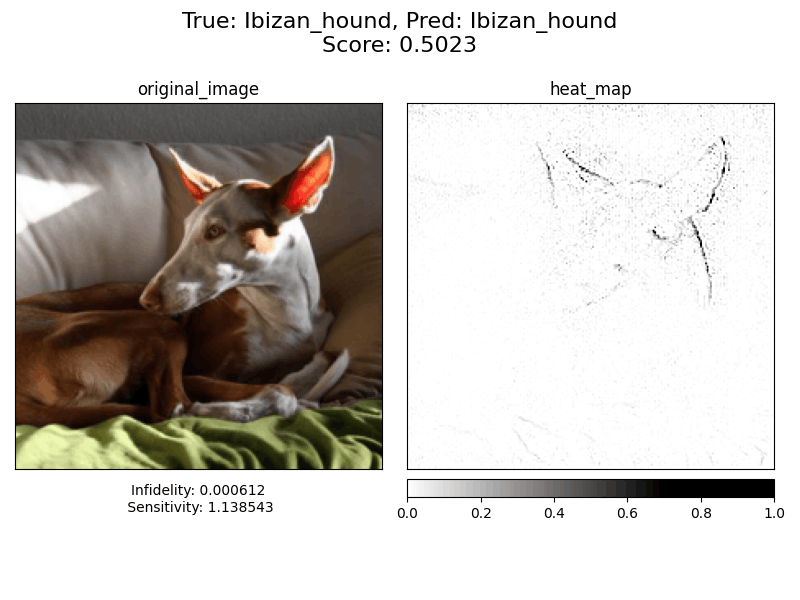
\includegraphics[width=0.50\textwidth]{background/images/1280-Ibizan_hound-Ibizan_hound.png}
  \caption{Visualization of the attribution by the Guided GradCAM generated for the class \textit{ibizan\_hound}. Image source: \textit{Stanford Dogs} \cite{stanford-dogs}}\label{fig:gradcam-ibizan-hound}
  \vspace{-30mm}
\end{wrapfigure}


To better visualize the attribution, we can look at Figure \ref{fig:gradcam-ibizan-hound}. For predicting a class of \textit{ibizan\_hound}, each pixel of the input image was given a value that defined its attribution to the prediction. Pixels (features) with higher attribution could be considered "more important" in predicting that class. We can see that the pixels with the highest attribution values are the pixels at the edges of the dog's head and ears. 

\vspace{\baselineskip}

As in the case of interpretability versus explainability (section \ref{section:interpretability-def}), the is a lack of agreement on vocabulary. Attribution methods are often known as \textit{saliency methods}, \textit{feature relevance}, \textit{feature importance}, \textit{heatmaps}, \textit{neuron activations}, and \textit{saliency masks}.

\newpage

\section{Quantitative and Qualitative research}

The type of research can be divided into qualitative or quantitative \cite{creswell2002educational}. The qualitative type of research is often related to the observation and processing of non-numerical data. The contrast to qualitative research is called quantitative research, and  it relies on the numerical analysis of collected data. Interpretability of machine learning models is a human-centric field of study. That is why most of the XAI method researchers base their solutions on qualitative measures rather than quantitative ones. This thesis argues that the current qualitative approach can prone to errors.

\subsection{Qualitative measures}

In qualitative research, the data is collected through observation, pools, or interviews. This kind of data is very subjective and related to the person providing the data. An example of such a subjective measure is shown in Figure \ref{fig:attr-comparison}. If presented with two attributions for the same input image, the decision of which one is better may change with the person. This is even more likely when two attributions have similar "quality". 

\begin{figure}[h]
  \centering
 \begin{subfigure}{.23\textwidth}
    \centering
    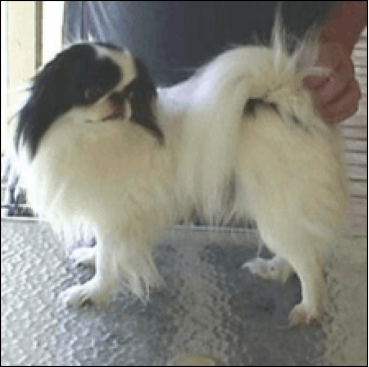
\includegraphics[width=\textwidth]{background/images/org-Japanese_spaniel.png}
    \caption{Input data}\label{fig:attr-comparision-image}
\end{subfigure}
 \begin{subfigure}{.23\textwidth}
    \centering
    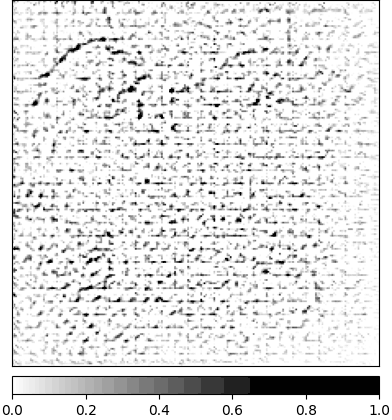
\includegraphics[width=\textwidth]{background/images/deconv-Japanese_spaniel.png}
    \caption{Attribution 1}\label{fig:attr-comparision-deconv}
\end{subfigure}
 \begin{subfigure}{.23\textwidth}
    \centering
    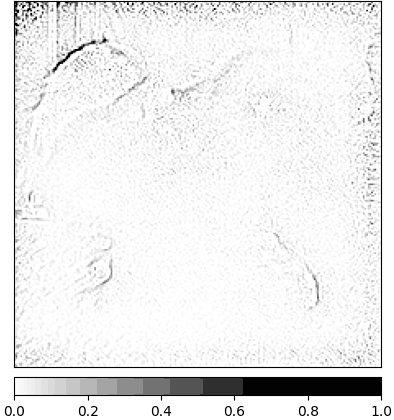
\includegraphics[width=\textwidth]{background/images/gbpJapanese_spaniel.png}
    \caption{Attribution 2}\label{fig:attr-comparision-gbp}
\end{subfigure}

 \caption{Comparison of attributions from two different methods for the same input data. Both attributions are generated for the same model with different XAI methods. Image source: \textit{Stanford Dogs} \cite{stanford-dogs} }\label{fig:attr-comparison}
\end{figure}

The results of the qualitative measures cannot be compared with each other without the specific context and prior knowledge about the data producers. Even with that knowledge, comparing the results might be difficult. The same issue applies to reproducibility, were to repeat the measurement, we have to be sure that all the participants are going to give the same answer. Another problem with qualitative measures is their scalability. Because most of the methods rely on human input, to measure the same method again or to compare it with another method, we have to repeat the work twice.

\subsection{Quantitative measures}

The data in the quantitative research is stored in a numeric form. This numeric form has to be comparable with other data measured in the same way. Each measurement is repeatable, and when done once, it can be reused all over again. This type of research has a huge advantage over qualitative research because of its scalability. The problem with qualitative measurement is that we have to define the measure to return meaningful results. Defining a measure of human visual perception is a difficult task, and the measure itself should be objective, which is even harder when trying to measure complex things like attributions. Having such a measure allows us to easily compare and reproduce experiments.

\newpage

\section{Related work}

Ghorbani et al. \cite{ghorbani2019interpretation} discuss attacks using adversarial perturbations to produce different interpretations of the same image. Their paper shows that we can generate such adversarial perturbations that produce perceptively indistinguishable inputs with the same prediction, but the attribution differs by a considerable margin from the original attribution. This thesis also focuses on the effect of input perturbation, but instead of searching for adversarial perturbation, it applies augmentations that aim to simulate real-world image processing that happens in modern cameras and check how they influence attribution.

\vspace{\baselineskip}

Another approach to the influence of perturbation on interpretability was taken by Kindermans et al. \cite{kindermans2016investigating}. They have studied the effect of applying noise to the input image and what effect it has on the explanation provided by the methods available at that time.

\vspace{\baselineskip}

One of the most influential papers on the subject was done by Adebayo et al. \cite{adebayo2018sanity} in 2018. Their work examined the influence of noise on the gradient values on different layers in the CNN. This was done by checking the correlation between the value of the gradient before and after applying the noise. The check was performed using multiple similarity metrics. Their work proved that gradients could be influenced by simple noise.

\vspace{\baselineskip}

Hooker et al. \cite{hooker2018benchmark} were one of the first who tried to measure the XAI methods quantitatively. The exact framework used is described in section \ref{section:roar}. The study assumed that if after removing pixels attributed as important to the prediction and retraining the model, the model still performs well, then the attribution is wrong. This approach might be logical, but it is extremely computationally expensive and therefore useless in real-world scenarios when there are limited resources.